\section{Taking derivatives}
Taking derivatives using the definitions quickly becomes unmanagable. Because of this,
we want to produce a set of rules which will allow us to take derivatives of common
functions.

\subsection{Differentiation of polynomials}
We begin with a few easy observations that will allow us to take derivatives of
polynomials.

\begin{thm}[Arithmetic of derivatives]
  Let $ f $ and $ g $ be functions.
  \begin{enumerate}
    \item If $ f(x) = \lambda $ for all $ x $ (where $ \lambda $ is a constant), then $ f'(x) = 0 $ for all $ x $.
    \item The derivative of $ f + g $ is $ f' + g' $ (i.e. for all $ x $, $ (f + g)'(x) = f'(x) + g'(x) $).
    \item If $ \lambda $ is a constant, then $ (\lambda f)' = \lambda f' $.
  \end{enumerate}
\end{thm}
\begin{proof}
  \begin{enumerate}
    \item In this case, $ \frac{f(x + h) - f(x)}{h} = \frac{\lambda - \lambda}{h} = 0 $, so the difference quotient is always zero and so is the derivative.
    \item If $ h $ is small, $ (f + g)(x + h) - (f + g)(x) =  f(x + h) + g(x + h) - f(x) - g(x) \approx f'(x)h + g'(x)h $ and so the derivative at $ x $
          is $ f'(x) + g'(x) $.
    \item $ (\lambda f)(x + h) - (\lambda f)(x) = \lambda (f(x + h) - f(x)) \approx \lambda (f'(x) h) = (\lambda f')(x) h $.
  \end{enumerate}
\end{proof}

Now we consider $ f(x) = x^n $ for integers $ n $. Using the binomial theorem,
\begin{displaymath}
  \lim_{h \to 0} \frac{f(x + h) - f(x)}{h} = \lim_{h \to 0} \frac{(x + h)^n - x^n}{h} = \lim_{h \to 0} \frac{x^n + n x^{n - 1} h + \cdots - x^n}{h}
\end{displaymath}
where every term hidden in the $ \cdots $ includes an $ h^2 $ factor, so we obtain
\begin{equation}
  f'(x) = \lim_{h \to 0} n x^{n - 1} + h(\cdots) = nx^{n - 1}.
\end{equation}
In fact, although we proved this for integer $ n $, it holds in general:
\begin{thm}[Power law]
  If $ f(x) = x^\alpha $ then $ f'(x) = \alpha x^{\alpha - 1} $.
\end{thm}

\begin{ex}
  We can now differentiate every function of the form $ f(x) = a_1 x^{b_1} + \cdots + a_n x^{b_n} $: $ f'(x) = b_1 a_1 x^{b_1 - 1} + \cdots + b_n a_n x^{b_n - 1} $.
  In particular, if $ f(x) = \sqrt{x} $ then $ f'(x) = \frac{1}{2\sqrt{x}} $; if $ g(x) = 2x^2 + 3 $ then $ g'(x) = 4x $; and if $ h(x) = \frac{1}{x} + x^7 $
  then $ h'(x) = -\frac{1}{x^2} + 7x^6 $.
\end{ex}

\subsection{Trigonometric derivatives}
We have already seen that $ \sin' = \cos $; using similar reasoning, we can prove the following:
\begin{thm}[Trigonometric derivatives]
  \def\arraystretch{1.5}
  \begin{tabular}{|c|c|l|}\hline
    \textbf{Function} & \textbf{Derivative} \\\hline
    $ \sin x $ & $ \cos x $\\\hline
    $ \cos x $ & $ -\sin x $\\\hline
    $ \tan x $ & $ \sec^2 x $\\\hline
    $ \csc x $ & $ -\csc x \cot x $\\\hline
    $ \sec x $ & $ \sec x \tan x $\\\hline
    $ \cot x $ & $ -\csc^2 x $\\\hline
  \end{tabular}
\end{thm}

I will use the result $ \sin' = \cos $ to prove that $ \cos' = -\sin $, and we will prove
the rest at a later time. Indeed, $ \cos x = \sin (x + \pi/2) $; then $ \od{}{x} \cos x = \od{}{x} \sin(x + \pi/2) $.
But the graph of $ \sin(x + \pi/2) $ is just the graph of $ \sin x $, shifted to the left
by $ \pi/2 $. Hence the slope of $ \sin (x + \pi/2) $ is the same as the slope of $ \sin x $,
but shifted to the left by $ \pi/2 $; and the slope of $ \sin x $ is $ \cos x $. Hence:
\begin{equation}
  \od{}{x} \cos x = \od{}{x} \sin(x + \pi/2) = \cos(x + \pi/2) = -\sin x.
\end{equation}
(This little trick I used here is explored in more detail in the L2 notes; we don't need it
too often this year, because in a couple of sections we will learn a much more general way
of dealing with this kind of situation.)

\begin{app}
  Many phenomena in physics can be modelled with sine waves; for example, if a particle on the end of a spring
  is moving with simple harmonic motion, then it has position $ x = A \sin (\omega t + \phi) $; taking derivatives,
  we find that it has velocity $ v = \od{x}{t} = A\omega \cos (\omega t + \phi) $ and acceleration $ a = \od[2]{x}{t} = -A \omega^2 \sin (\omega t + \phi) $.
  In other words, it is always accelerating in the opposite direction to its movement!
\end{app}

\subsection{Exponential functions}
The next function we want to consider here is $ f(x) = a^x $, for constants $ a $. We can
compute that
\begin{displaymath}
  f'(x) = \lim{h \to 0} \frac{a^{x + h} - a^x}{h} =  a^x \lim_{h \to 0} \left( \frac{a^h - 1}{h} \right).
\end{displaymath}
So the exponential functions $ a^x $ have derivatives of the form $ Ka^x $, where $ K $ is some constant. This
begs the question, for which value of $ a $ (if any) does $ \od{}{x} a^x = a^x $ (i.e. $ K = 1 $)? Well, we
need to solve
\begin{displaymath}
  \lim_{h \to 0} \left( \frac{a^h - 1}{h} \right) = 1
\end{displaymath}
for $ a $. We will begin by setting $ u = 1/h $, so when $ h \to 0 $ we have $ u \to \infty $. Thus
\begin{displaymath}
  \lim_{u \to \infty} (a^{1/u} - 1)u = 1 = \lim_{u \to \infty} 1;
\end{displaymath}
and applying the limit laws,
\begin{align*}
  \lim_{u \to \infty} (a^{1/u} - 1) &= \lim_{u \to \infty} \frac{1}{u};\\
  \lim_{u \to \infty} a^{1/u} &= \lim_{u \to \infty} \frac{1}{u} + 1;\\
  a = \lim_{u \to \infty} (a^{1/u})^u &= \lim_{u \to \infty} \left(\frac{1}{u} + 1\right)^u.
\end{align*}
It can be shown fairly easily that $ \lim_{u \to \infty} \left(\frac{1}{u} + 1\right)^u $ does
indeed exist (it has a value of $ 2.71828... $), and we define its value to be $ e $. Thus $ e $
is the base for the exponential function that is its own derivative: $ \od{}{x} e^x = e^x $. Often,
we write $ \exp(x) := e^x $.

Finally, note that if $ K = \lim_{h \to 0} \left( \frac{a^h - 1}{h} \right) = \lim_{u \to \infty} u(a^{1/u} - 1) $ then
\begin{displaymath}
  a = \lim_{u \to \infty} \left(\frac{K}{u} + 1\right)^u = \lim_{u \to \infty} \left(\left(\frac{K}{u} + 1\right)^{u/K}\right)^K = \lim_{(u/K) \to \infty} \left(\left(\frac{K}{u} + 1\right)^{u/K}\right)^K = e^K;
\end{displaymath}
hence $ \od{}{x} a^x = a^x K = a^x \log_e a $. (We normally write $ \log_e = \ln $.)

\subsection{Logarithmic derivatives}
Finally, let us calculate $ \od{}{x} \ln x $. (This will allow us to find $ \od{}{x} \log_a x $ for all $ a $, using the
relationship $ \log_a x = \frac{1}{\ln a} \ln x $.)

\begin{displaymath}
  \ln'(x) = \lim_{h \to 0} \frac{\ln(x + h) - \ln(x)}{h} = \lim_{h \to 0} \frac{1}{h} \ln\left(1 - \frac{h}{x} \right) = \lim_{h \to 0} \ln\left(1 - \frac{h}{x} \right)^{1/h}
\end{displaymath}
Let $ u = 1/h $; so as $ h \to 0 $, $ u \to \infty $. Then, substituting, we obtain
\begin{displaymath}
  \ln'(x) = \lim_{u \to \infty} \ln \left( 1 - \frac{1}{ux} \right)^u.
\end{displaymath}
Now, we use the fact that $ \exp(\ln x) = x $:
\begin{displaymath}
  e^{\ln'(x)} = \lim_{u \to \infty} \exp(\ln \left( 1 - \frac{1}{ux} \right)^u) = \lim_{u \to \infty}\left( 1 - \frac{1}{ux} \right)^u
              = \lim_{u \to \infty} \left(\left( 1 - \frac{1}{ux} \right)^{ux}\right)^{(1/x)}
              = e^{1/x}
\end{displaymath}
and thus $ \ln'(x) = 1/x $.

\subsection{Exercises and Problems}
\begin{enumerate}
  \item Find the derivatives of $ 3x^3 $, $ 2x^2 $, and $ 6x^5 $. Conclude that $ (fg)' \neq f' g' $ in general.
  \item Find the derivatives of the following functions with respect to $ t $:
    \begin{enumerate}
      \item $ y = 2t^3 + 3t^2 $
      \item $ y = \sqrt{t} $
      \item $ y = (2t + 1)(t - 4) $
      \item $ g(t) = 4 \sec t + 9 \tan t $
      \item $ h(t) = \sqrt[5]{t} + 2\csc t - \ln t^3 $
      \item $ \phi'(t) = \csc x + 12x^{1273} + 9 $
      \item $ y = 2017t^{2016} + (t + 2)^2 $
      \item $ y = 940\sin t + \frac{1}{2}e^{t + 2} $
    \end{enumerate}
  \item Where is the function $ x \mapsto x^3 - 2x^2 - x + 1 $ increasing?
  \item Find the velocity $ v $ of a particle at time $ t = 2\pi $ if its position function for $ t > 0 $ is $ x = e^t - \sin t $.
  \item Find the slope of the tangent line to $ y = x + \tan x $ at $ (\pi, \pi) $.
  \item Find a linear approximation $ \tilde f $ to $ f(x) = x^2 + x + 1 $ at $ (0,1) $, and find some $ \delta $ such
        that for all $ x $ satisfying $ -\delta < x < \delta $, $ -0.1 < \tilde f(x) - f(x) < 0.1 $.
  \item It is \textbf{not} true that the derivative of $ f(g(x)) $ is $ f'(g'(x)) $.
    \begin{enumerate}
      \item For a counterexample, consider $ f(x) = x^2 $ and $ g(x) = x $; show that $ f'(g'(x)) = 2 $, but $ \od{}{x} f(g(x)) = 2x $.
      \item Compute the derivative of $ \ln x^2 $.
    \end{enumerate}
  \item Suppose the derivative of a function is $ \od{y}{x} = 3x^2 - x - 4 $. What could the original function be?
  \item Find the 64th derivative of $ \sin x $.
  \item Find the $ n$th derivative of $ x^n $.
  \item If $ y = 2\sin 3x \cos 2x $, find $ \od{y}{x} $. (Hint: use an identity to rewrite this as a sum of functions.)
  \item For which values of $ x $ does the graph of $ f(x) = x + 2\sin x $ have a horizontal tangent?
  \item Show that $ y = 6x^3 + 5x - 3 $ has no tangent line with a slope of 4.
  \item Find real values of $ \alpha $ and $ \beta $ such that, if $ y = \alpha \sin x + \beta \cos x $,
        then $ y'' + y' -2y = \sin x $.
  \item Consider a \SI{12}{\metre} long ladder leaning against a wall such that the top of the ladder makes an
        angle $ \theta $ with the wall. If this angle $ \theta $ is varied, the distance $ D $ between the bottom
        of the ladder and the wall also changes. If $ \theta = \pi/3 $, what is the rate of change of $ D $ with
        respect to $ \theta $?
  \item Prove that the function $ \varphi $ given by $ \varphi(x) = \frac{x^{101}}{101} + \frac{x^{51}}{51} + x + 1 $
        never has a horizontal tangent line.
  \item The derivative is primarily a geometric concept, not an algebraic one.
    \begin{enumerate}
      \item The area of a circle of radius $ r $ is $ A = \pi r^2 $. Find $ \od{A}{r} $. What do you notice?
      \item Explain item (a) geometrically.
      \item The volume of a sphere is given by $ V = \frac{4}{3} \pi r^3 $. Find an expression for the surface area.
    \end{enumerate}
\end{enumerate}

\subsection{References}
See sections 2.1 -- 2.4 of Stewart. For a discussion of the exponential function and its
relationship to compound interest and rates of growth, see Thompson chapter XIV.

\subsection{Homework}
\paragraph{Reading}
The number $ e \approx 2.718 $ is known as Euler's number, after the Swiss mathematician Leonhard Euler.

\begin{center}
  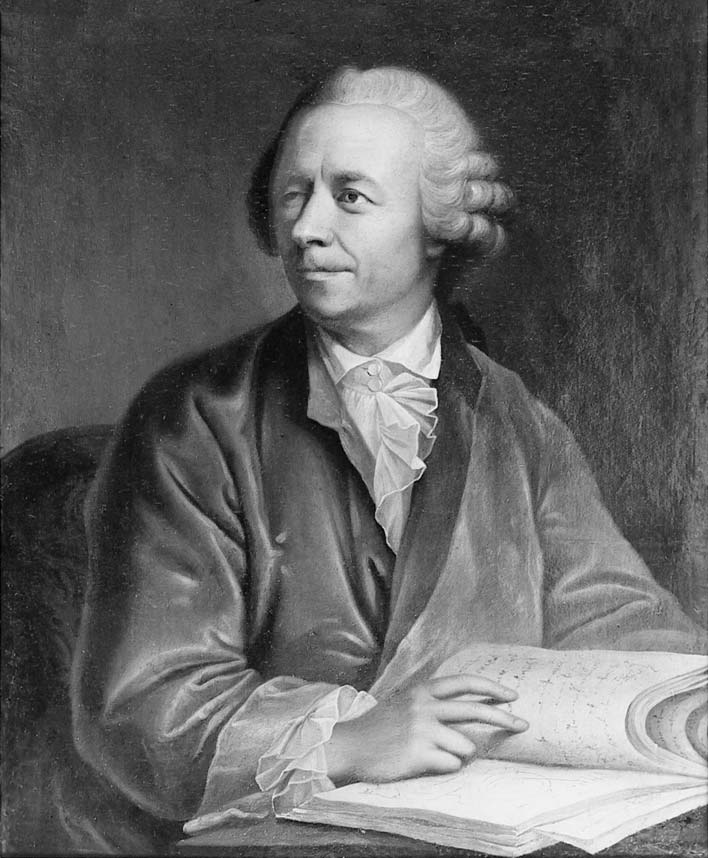
\includegraphics[width=0.2\textwidth]{euler}
\end{center}

Leonhard Euler (1707--1783) was Switzerland's foremost scientist and one of the three greatest mathematicians of modern times (the other two being
Gauss and Riemann).

He was perhaps the most prolific author of all time in any field. From 1727 to 1783 his writings poured out in a seemingly endless flood, constantly
adding knowledge to every known branch of pure and applied mathematics, and also to many that were not known until he created them. He averaged about
800 printed pages a year throughout his long life, and yet he almost always had something worthwile to say and never seems long-winded. The publication
of his complete works was started in 1911, and the end is not in sighr: it is now esitmated that 100 large volumes will be required for completion
of the project. He suffered blindess during the last 17 years of his life, but with the aid of his powerful memory and fertile imagination, and with
helpers to write his books and papers from dictation, he actually increased the already prodigious output of work.

Though he was not himself a teacher Euler has had a deeper influence on the teaching of mathematics than any other person. This came about chiefly
through his three great treatises: \emph{Introductio in Analysin Infinitorum} (1748); \emph{Institutiones Calculi Differentialis} (1755);
and \emph{Institutiones Calculi Integralis} (1768--1794). There is considerable truth in the old saying that all elementary and advanced calculus
textbooks since 1748 are essentially copies of Euler or copies of copies of Euler. These works summed up and codified the discoveries of his
predecessors, and are full of Euler's own ideas. He extended and perfected plane and solid analytic geometry, introduced the analytic approach
to trigonometry, and was responsible for the modern treatment of the functions $ \ln $ and $ \exp $. It was though his work that the symbols $ e $,
$ \pi $, and $ i $ became common currency for all mathematicians, as well as the functions $ \sin $ and $ \cos $.

He was the first and greatest master of infinite series, products, and fractions; in 1736, he made the wonderful discovery that
\begin{displaymath}
  1 + \frac{1}{4} + \frac{1}{9} + \frac{1}{16} + \cdots = \frac{\pi^2}{6},
\end{displaymath}
and also found the sums of the reciprocals of the fourth and sixth powers. (A closed form for the sum of the reciprocals of the
cubes is still unknown.)

The foundations of classical mechanics had been laid down by Newton, but Euler was the principle architect. In his treatise of 1736
he was the first to explicitly introduce the concept of a point-like particle, and he was the also the first to study the acceleration
of a particle moving along any curve and to use the notion of a vector in connection with velocity and acceleration. His continued
successes in mathematical physics were so numerous, and his influence was so pervasive, that most of his discoveries are not credited
to him at all and are taken for granted by physicists as part of the natural order of things.

\begin{flushright}
  Adapted from \textit{Differential equations with applications and historical notes} (pp.136--146) by George F. Simmons (McGraw-Hill, 1991).
\end{flushright}


\paragraph{Problems}
\begin{enumerate}
  \item Differentiate with respect to $ x $:
    \begin{enumerate}
      \item $ x^2 + \frac{1}{x} $
      \item $ tx^t $
      \item $ \sin x - \cos x $
      \item $ \sqrt[5]{x^4} $
    \end{enumerate}
  \item Explain why you cannot use the power rule to find the derivative of $ x^x $.
  \item Find the $ n$th derivative of $ \frac{1}{x^n} $.
  \item Suppose a population grows exponentially with time, such that after $ t $ years the population is $ P(t) = P_0 + 10^t $.
    \begin{enumerate}
      \item Find the rate of change of the population at $ t = 100 $.
      \item Explain why this population model is unrealistic.
    \end{enumerate}
\end{enumerate}
